\documentclass[a4]{article}

% PACKAGES %%%%%%%%%%%%%%%%%%%%%%%%%%%%%%%%%%%%%%%%%%%%%%%%%%%%%%%%%%%%%%%%%%%%%
\usepackage[utf8]{inputenc}
\usepackage{framed}
\usepackage{makecell}
\usepackage[english]{babel}

\usepackage{url}

%!TEX encoding = UTF-8 Unicode

\setlength{\textwidth}{6.5 in}
\setlength{\textheight}{8.5 in}
\setlength{\headsep}{0.5 in}

\usepackage{multirow, array}
\usepackage{float}
\usepackage{charter}

\usepackage[breaklinks=true]{hyperref}

\usepackage{amsmath,longtable,siunitx, float, graphicx, dcolumn, bm, fancyhdr, subcaption, caption, multicol, setspace}
\usepackage{amssymb}

\usepackage[hmarginratio=1:1, top=32mm, columnsep=20pt, headsep=\dimexpr20mm, margin=0.8in, top=1in ]{geometry}
\usepackage{comment}
\usepackage{booktabs}
\usepackage{enumitem}
\usepackage{tabularx}
\usepackage[table]{xcolor} % [table] provides \cellcolor (loads colortbl)

\usepackage{tikz}
\usetikzlibrary{shapes.geometric, arrows.meta, positioning}

% ----------- global tikz styles (matches the CV challenge docs) -----------
\tikzset{
  font=\scriptsize,
  every node/.style       = {transform shape},
  startstop/.style        = {ellipse, draw, fill=blue!10,
                             inner sep=2pt, minimum width=16mm, align=center},
  process/.style          = {rectangle, draw, fill=orange!15,
                             text width=24mm, inner sep=3pt, align=center},
  data/.style             = {rectangle, draw, fill=green!12, rounded corners,
                             text width=24mm, inner sep=3pt, align=center},
  arrow/.style            = {->, >=Stealth, shorten >=1pt, shorten <=1pt}
}

% Colours for the schedule
\definecolor{heavyweek}{HTML}{FFE8CC}
\definecolor{phase0}{HTML}{D9E8FB}
\definecolor{phase1}{HTML}{DDF4DD}
\definecolor{phase2}{HTML}{F3DDF4}
\definecolor{bufferc}{HTML}{EFEFEF}

\newcommand{\TODO}{\textbf{\textcolor{red}{TODO}}}
\newcommand{\deliv}[1]{\textit{\textbf{Deliverable:} #1}}

\renewcommand{\thesection}{\Roman{section}}

% ----------- header / footer (logos optional, guarded) -----------
\pagestyle{fancy}
\fancyhf{}
\lhead{\IfFileExists{CETIC.png}{\includegraphics[scale=0.4]{CETC.png}}{\small\textbf{CETC}}}
\rhead{\IfFileExists{Cornell-University-Logo.png}{\includegraphics[scale=0.025]{Cornell-University-Logo.png}}{\small Cornell University}}
\cfoot{\thepage}
\renewcommand{\headrulewidth}{0.4pt}
\renewcommand{\footrulewidth}{0pt}

\begin{document}

\thispagestyle{fancy}

\begin{center}
    \textbf{\large Orbit Odyssey -- Natural Language Processing} \\
    {Week-by-Week Project Plan}

    \vspace{0.7em}

    David Alejandro Fuquen \\

    {\small Planning horizon: 21 September 2025 -- 15 November 2025} \\
    {\small \today}
\end{center}

\vspace{0.5em}

% =====================================================================
\begin{center}
\begin{minipage}{0.92\linewidth}
\itshape
While charting a distant sector on a deep-space expedition, our crew intercepts a
mysterious transmission --- a message written in an alien language we have never
seen before. Arriving with it are a few scattered fragments of a ``Rosetta Stone.''
To understand the message, and to answer it, we must teach our onboard computer to
read the alien words and turn them into commands our robot can follow.
\end{minipage}
\end{center}

\vspace{0.6em}

% =====================================================================
\section{Overview}

This challenge turns that story into a hands-on lesson in how computers work with
language. Students discover how a computer takes everyday human language --- and
even a completely unknown alien one --- and turns it into clear instructions a robot
can follow. It runs in two phases:

\begin{itemize}[leftmargin=*]
    \item \textbf{Phase 1 -- English.} Students read a casual ``mission log''
    and teach the computer to turn it into a simple list of robot commands
    (for example: move forward, then turn right).
    \item \textbf{Phase 2 -- Alien language.} Stranded in space, the crew receives
    a distress message in an unknown alien language, along with a partial
    ``Rosetta Stone.'' Students use it to decode the message and recover the
    commands hidden inside.
\end{itemize}

\noindent\textbf{The key takeaway.} The alien language makes the main lesson
impossible to miss: the computer never truly ``understands'' words like
\emph{move} or \emph{forward}. It simply recognizes patterns and matches them using
the Rosetta Stone --- exactly what it was doing in English all along, where it only
looked like real understanding.

% =====================================================================
\begin{comment}
\section{Locked Design Decisions}\label{sec:decisions}

The following were agreed during planning and frame every task below.

\begin{center}
\renewcommand{\arraystretch}{1.3}
\begin{tabularx}{\linewidth}{@{}p{3.4cm}X@{}}
\toprule
\textbf{Decision} & \textbf{Resolution} \\
\midrule
Web platform &
Rebuild the current Streamlit prototype as a \textbf{standalone Next.js web
application} (browser-accessible, no local Python install for students). \\

NLP approach &
A \textbf{small, genuinely trainable intent~+~slot model} that students train
themselves --- mirroring the ``train your own model'' arc of the CV challenge,
rather than a hand-written rule table. \\

Robot execution &
\textbf{Out of scope.} The deliverable is the extracted \emph{command list}
that \emph{would} be handed to the XRP. No serial/hardware integration. \\

Alien language &
A \textbf{fixed constructed mini-grammar} (novel vocabulary, distinct word
order/morphology) with a \textbf{partial Rosetta Stone}, and
\textbf{per-session relexification} (swap surface word-forms per team) for
replayability and anti-cheat. \\
\bottomrule
\end{tabularx}
\end{center}

\section{System Architecture}

\subsection*{Target stack}
\begin{itemize}[leftmargin=*]
    \item \textbf{Next.js (App Router)} single application: student-facing UI plus
    lightweight API routes for content, seeds, and answer-key checks.
    \item \textbf{In-browser training with TensorFlow.js} as the recommended model
    runtime: students watch loss/accuracy update live (echoing the CV challenge's
    WebSocket progress), and no GPU server is required. \emph{Fallback:} a small
    Python/FastAPI training microservice if a heavier model proves necessary
    (open question, \S\ref{sec:open}).
    \item \textbf{Domain logic in TypeScript}, ported from the Streamlit prototype:
    tokenizer, command grammar, and the existing 2D path simulator (reused only as
    an optional auto-grader, not for robot control).
\end{itemize}

\subsection*{The model (shared across both phases)}
\begin{itemize}[leftmargin=*]
    \item \textbf{Intent classifier}: per clause, predict the action
    (\texttt{MOVE} / \texttt{TURN}; optionally \texttt{STOP} later).
    \item \textbf{Slot extractor}: token-level tagging for the numeric amount and
    direction (e.g.\ tiles, degrees, left/right), assembled into the final command.
    \item \textbf{Training data}: an authored, augmented parallel corpus
    (sentence $\rightarrow$ command). In Phase 2 the \emph{same} architecture is
    retrained on the Rosetta correspondence over alien tokens.
\end{itemize}

\subsection*{Pipeline}
\begin{center}
\begin{tikzpicture}[node distance=6mm and 9mm]
  \node[data]     (msg)   {Mission log / \\ alien message};
  \node[process]  (tok)   [right=of msg]  {Tokenize};
  \node[process]  (intent)[right=of tok]  {Intent \\ classify};
  \node[process]  (slot)  [right=of intent]{Slot \\ extract};
  \node[startstop](cmd)   [right=of slot]  {Command \\ list};
  \draw[arrow] (msg)--(tok);
  \draw[arrow] (tok)--(intent);
  \draw[arrow] (intent)--(slot);
  \draw[arrow] (slot)--(cmd);
  \node[data] (rosetta) [below=8mm of intent] {Training data / \\ Rosetta Stone};
  \draw[arrow] (rosetta) -- (intent);
  \draw[arrow] (rosetta) -| (slot);
\end{tikzpicture}
\end{center}

    
\end{comment}

% =====================================================================


% =====================================================================
\section{Phase Map}

\begin{center}
\renewcommand{\arraystretch}{1.3}
\begin{tabularx}{\linewidth}{@{}p{3.2cm}p{3.4cm}X@{}}
\toprule
\textbf{Phase} & \textbf{Weeks} & \textbf{Outcome} \\
\midrule
\cellcolor{phase0}Setup &
Wk 1 (Sep 21--27) &
Move the current prototype onto a proper, easy-to-access web application. \\

\cellcolor{phase1}Phase 1 -- English &
Wk 2--4 (Sep 28--Oct 18) &
Students teach the computer to turn English mission logs into robot commands. \\

\cellcolor{phase2}Phase 2 -- Alien &
Wk 5--7 (Oct 19--Nov 8) &
Students decode an alien message into robot commands using a partial Rosetta Stone. \\

\cellcolor{bufferc}Delivery &
Wk 8 (Nov 9--15) &
Guides, testing, final polish, and hand-off. \\
\bottomrule
\end{tabularx}
\end{center}

% =====================================================================
\section{Week-by-Week Plan}

\begin{center}
\renewcommand{\arraystretch}{1.5}
\begin{tabularx}{\linewidth}{@{}p{1.1cm}p{2.6cm}X@{}}
\toprule
\textbf{Wk} & \textbf{Dates} & \textbf{General goal for the week} \\
\midrule
\cellcolor{phase0}1 & Sep 21--27 & Set up the web application and move the current prototype onto it. \\
\cellcolor{heavyweek}\textbf{2} & \textbf{Sep 28--Oct 4} & \textbf{Main build week.} Build the core English experience: students train the computer to turn a mission log into robot commands. \\
\cellcolor{phase1}3 & Oct 5--11 & Continue building the English experience until it runs smoothly end to end. \\
\cellcolor{phase1}4 & Oct 12--18 & Refine and finalize the English challenge, including how student results are scored. \\
\cellcolor{phase2}5 & Oct 19--25 & Create the alien language and its partial Rosetta Stone decoding key. \\
\cellcolor{phase2}6 & Oct 26--Nov 1 & Build the alien challenge so students can decode a message into robot commands. \\
\cellcolor{phase2}7 & Nov 2--8 & Add scoring, teacher tools, and a unique language per team to keep the challenge fair. \\
\cellcolor{bufferc}8 & Nov 9--15 & Write the guides, run final checks, publish the application, and deliver. \\
\bottomrule
\end{tabularx}
\end{center}

\noindent \textbf{Why the second week carries the most.} The week of
\textbf{28 September--4 October} is when I am most available: my students are on
Fall break, so I can dedicate my class time to the project. The heaviest and most
important work --- building the core English experience --- begins there and
continues into the following week. The final week (Nov 9--15) is reserved for
delivery, and also acts as a safety buffer in case earlier weeks run long.

% =====================================================================

% =====================================================================

% =====================================================================
\begin{comment}

\section{Milestones and Dependencies}

\begin{center}
\renewcommand{\arraystretch}{1.25}
\begin{tabularx}{\linewidth}{@{}p{1.2cm}p{3.2cm}X@{}}
\toprule
\textbf{By} & \textbf{Milestone} & \textbf{Depends on} \\
\midrule
Sep 27 & M0: Next.js skeleton runs; logic ported & --- \\
Oct 4  & M1: English phase end-to-end (heavy week) & M0 \\
Oct 11 & M2: English phase finalized \& scored & M1 \\
Oct 18 & M3: Alien language + Rosetta generator & (independent; can start early) \\
Oct 25 & M4: Alien phase integrated & M2, M3 \\
Nov 1  & M5: Scoring + moderator + anti-cheat & M4 \\
Nov 8  & M6: Docs + pilot test complete & M5 \\
Nov 15 & M7: Deployed \& delivered & M6 \\
\bottomrule
\end{tabularx}
\end{center}

\noindent\textbf{Critical path:} M0 $\rightarrow$ M1 $\rightarrow$ M2 $\rightarrow$
M4 $\rightarrow$ M5 $\rightarrow$ M6 $\rightarrow$ M7. The alien-language
\emph{design} (M3) has no dependency on the model and can be pulled earlier if a
week frees up. Phase 2 \emph{integration} (M4) does depend on the finished Phase 1
model, since it reuses the same architecture.


\section{Risks and Mitigations}

\begin{center}
\renewcommand{\arraystretch}{1.25}
\begin{tabularx}{\linewidth}{@{}p{4.6cm}X@{}}
\toprule
\textbf{Risk} & \textbf{Mitigation} \\
\midrule
In-browser training is slow or unstable &
Keep the model tiny with a fixed vocabulary; spike it in Week 1; fall back to a
small Python/FastAPI training microservice if needed. \\

Model doesn't convincingly show ``no understanding'' &
Design the corpus so shallow patterns suffice; add an explicit reflection step
comparing English vs.\ alien behaviour. \\

Alien language too hard or too easy &
Validate solvability by hand in Week 4; tune Rosetta Stone coverage; pilot in
Week 7. \\

Only one high-availability week &
Front-load the riskiest work (model + end-to-end loop) into Week 2; keep Week 8
as an explicit buffer. \\

Scope creep toward robot control &
Command list is the hard boundary; XRP integration stays out of scope. \\
\bottomrule
\end{tabularx}
\end{center}

% =====================================================================
\section{Definition of Done}

\begin{itemize}[leftmargin=*, itemsep=1pt]
    \item A student can, in a browser, train the model and decode both an English
    mission log and an alien transmission into a correct \textbf{command list}.
    \item Each team receives a \textbf{relexified} alien language from a seed, with
    a solvable partial Rosetta Stone and a verifiable answer key.
    \item Moderators can assign seeds, grade submissions, and export command lists.
    \item \textbf{Student Guide} and \textbf{Moderator Guide} exist (LaTeX, CV style).
    \item The app is deployed and reachable; both phases pass QA by 15 November.
\end{itemize}

\section{Open Questions / Decisions Pending}\label{sec:open}

These do not block the start of Week 1 but should be resolved by the week noted.

\begin{enumerate}[leftmargin=*, itemsep=1pt]
    \item \textbf{Model runtime} (by Wk 1): confirm TensorFlow.js in-browser vs.\ a
    small Python/FastAPI training microservice.
    \item \textbf{Hosting} (by Wk 6): Vercel / self-host / fully offline classroom
    build?
    \item \textbf{Accounts \& persistence} (by Wk 3): session-local only, or reuse
    the CV app's auth/accounts?
    \item \textbf{Command vocabulary} (by Wk 2): just \texttt{MOVE}/\texttt{TURN},
    or also \texttt{STOP}/\texttt{GRAB}/etc.?
    \item \textbf{Number \& angle handling} (by Wk 2): integers, word-numbers,
    quarter/half-turn phrasing --- how far do we go?
    \item \textbf{Language of the ``known'' phase} (by Wk 3): English only, or also
    Spanish, given the CETC/Cornell context?
    \item \textbf{Assessment model} (by Wk 6): individual vs.\ team; leaderboard?
    \item \textbf{Branding} (by Wk 7): share the CV challenge's look/identity, or a
    distinct NLP identity?
\end{enumerate}
    
\end{comment}


\end{document}
